
Muchos sitios web intentan comparar las preferencias de dos usuarios para realizar sugerencias a partir de las preferencias de usuarios con gustos similares a los nuestros. Dado un ranking de $n$ productos (p.ej. pel\'iculas) mediante el cual los usuarios indicamos nuestras preferencias, un algoritmo puede medir la similitud de nuestras preferencias contando el n\'umero de inversiones: dos productos $i$ y $j$ est\'an \"invertidos\" en las preferencias de $A$ y $B$ si el usuario $A$ prefiere el producto $i$ antes que el $j$, mientras que el usuario $B$ prefiere el producto $j$ antes que el $i$. Esto es, cuantas menos inversiones existan entre dos rankings, m\'as similares ser\'an las
preferencias de los usuarios representados por esos rankings.

Por simplicidad podemos suponer que los productos se pueden identificar mediante enteros
$1, \cdots, n$, y que uno de los rankings siempre es $1,\cdots, n$ (si no fuese as\'i bastar\'ia reenumerarlos) y el otro es $a_1, a_2, \cdots, a_n$, de forma que dos productos $i$ y $j$ est\'an invertidos si $i < j$ pero $a_i > a_j$.
De esta forma nuestra representaci\'on del problema ser\'a un vector de enteros $v$ de tamaño $n$, de forma que $v[i] = a_i\ / \ i = 1, \cdots, n$.

El objetivo es diseñar, analizar la eficiencia e implementar un algoritmo \"divide y vencer\'as\" para medir la similitud entre dos rankings. Compararlo con el algoritmo de \"fuerza bruta\" obvio. Realizar tambi\'en un estudio emp\'irico e h\'ibrido de la eficiencia de ambos algoritmos.

\subsection{Automatizando el problema}
A la hora de generar los ejecutables, los datos y las gráficas hemos usado los siguientes scripts:

\begin{center}
	script.sh
\end{center}

\begin{lstlisting}[language=bash]
#!/bin/bash

if [ $# -ne 1 ]
then
    echo "Uso: $0 <nombre>"
    exit 1
fi

mkdir ../Graficas 2> /dev/null
mkdir ../Datos 2> /dev/null

# Fuerza bruta
g++ -std=c++11 -D GP_OUT ../src/fuerza_bruta.cpp
nelementos=10
echo "" > datos.dat
while [ $nelementos -lt 5000 ]; do
    ./a.out $nelementos >> datos.dat
    let nelementos=nelementos+10
done
gnuplot ./gnuplot/fuerza_bruta.gp

mv grafica.png ../Graficas/fuerza_bruta_$1.png
mv datos.dat ../Datos/fuerza_bruta_$1.dat
mv fit.log ../Datos/fit_fuerza_bruta_$1.log
echo "Fuerza bruta completado"

# DyV
g++ -std=c++11 -D GP_OUT ../src/dyv.cpp
nelementos=10
echo "" > datos.dat
while [ $nelementos -lt 5000 ]; do
    ./a.out $nelementos >> datos.dat
    let nelementos=nelementos+10
done
gnuplot ./gnuplot/dyv.gp

mv grafica.png ../Graficas/dyv_$1.png
mv datos.dat ../Datos/dyv_$1.dat
mv fit.log ../Datos/fit_dyv_$1.log
echo "DyV completado"

\end{lstlisting}

Para conseguir los datos y gr\'aficas hemos usado:

\begin{center}
	$fuerza_bruta.gp$
\end{center}

\begin{lstlisting}[language=gnuplot]
set terminal pngcairo
set output "grafica.png"

set title "Fuerza bruta"
set xlabel "Tamanio del vector"
set ylabel "Tiempo (s)"
set fit quiet
f(x) = a*x*x + b*x + c
fit f(x) "datos.dat" via a, b, c
plot "datos.dat", f(x)
\end{lstlisting}


\begin{center}
	dyv.gp
\end{center}

\begin{lstlisting}[language=gnuplot]
set terminal pngcairo
set output "grafica.png"

set title "Divide y vencer\'as"
set xlabel "Tamanio del vector"
set ylabel "Tiempo (s)"
set fit quiet
f(x) = a*x*x + b*x + c
fit f(x) "datos.dat" via a, b, c
plot "datos.dat", f(x)
\end{lstlisting}



\subsection{Fuerza bruta}
El programa usado para calcular los tiempos del algoritmo de fuerza bruta es:
\begin{lstlisting}[language=c++]
#include <iostream>
#include <vector>
#include <algorithm>
#include <ctime>
#include <cstdlib>
#include <chrono>
using namespace std;


int inversiones(vector<int> v){
  int count = 0;
  int size = v.size();
  for (int i=0; i < size; i++)
    for (int j=i+1; j < size; j++)
      if (v[i] > v[j])
        count++;

  return count;
}


int main(int argc, char** argv){
  if (argc < 2){
    cerr << "Formato " << argv[0] << " num_elem" << endl;
    return -1;
  }

  int n = atoi(argv[1]);
  vector<int> rankings(n);
  srandom(time(0));
  for (int i=0; i < n; i++)
    rankings[i] = i;

  random_shuffle(rankings.begin(), rankings.end());

  chrono::high_resolution_clock::time_point tantes, tdespues;
  chrono::duration<double> transcurrido;
  int n_inv;

  tantes = chrono::high_resolution_clock::now();
  n_inv = inversiones(rankings);
  tdespues = chrono::high_resolution_clock::now();

  transcurrido = chrono::duration_cast<chrono::duration<double>>(tdespues - tantes);

  #ifndef GP_OUT
    cout << "ranking: ";
    for (int i=0; i<n; i++)
      cout << rankings[i] << " ";
    cout << endl;
    cout << "Num inversiones: " << n_inv << endl;
  #else
    cout << n << " " << transcurrido.count() << endl;
  #endif

}
\end{lstlisting}

\begin{figure}[htb] 
\centering
	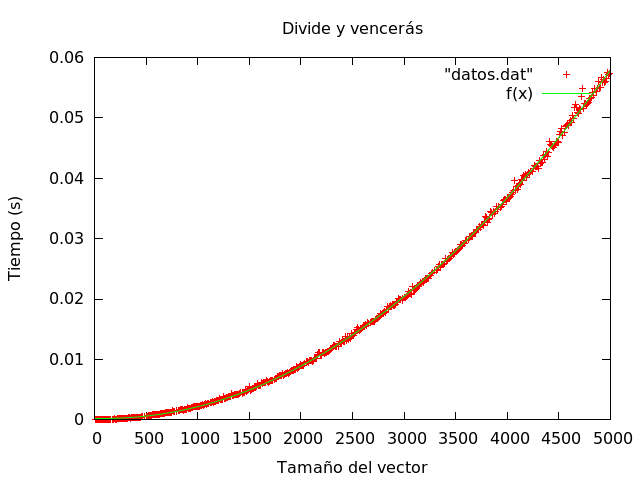
\includegraphics[width=0.6\textwidth]{../Opcional/Graficas/dyv_bruno.png}
	\caption{Subproblemas} 
	\label{fig:perros} 
\end{figure}


\subsection{Divide y vencer\'as}
El mismo problema usando un programa que utiliza divide y vencer\'as:

\begin{lstlisting}[language=c++]
#include <iostream>
#include <vector>
#include <algorithm>
#include <ctime>
#include <climits>
#include <cstdlib>
#include <chrono>
using namespace std;



/* ************************************************************ */
/*  M\'etodo de ordenaci\'on por mezcla  */

/**
   @brief Devuelve el numero de inversiones de un ranking.

   @param T: vector de elementos. Debe tener num_elem elementos.
             Es MODIFICADO.
   @param num_elem: n\'umero de elementos. num_elem > 0.

   @return el numero de inversiones

   Calcula el numero de inversiones aplicando el algoritmo de mezcla.
   Como consecuencia tambien ordena el vector T.
*/
inline static
int inversiones(int T[], int num_elem);



/**
   @brief Devuelve el n\'umero de inversiones de un ranking.

   @param T: vector de elementos. Tiene un n\'umero de elementos
                   mayor o igual a final. Es MODIFICADO.
   @param inicial: Posici\'on que marca el incio de la parte del
                   vector a ordenar.
   @param final: Posici\'on detr\'as de la \'ultima de la parte del
                   vector a ordenar.
		   inicial < final.

  Calcula el n\'umero de inversiones aplicando el algoritmo de mezcla.
  Como consecuencia tambien ordena el vector T.
*/
void inversiones_recursivo(int T[], int inicial, int final, int& num_inversiones);


/**
   @brief Ordena un vector por el m\'etodo de inserci\'on.

   @param T: vector de elementos. Debe tener num_elem elementos.
             Es MODIFICADO.
   @param num_elem: n\'umero de elementos. num_elem > 0.

   Cambia el orden de los elementos de T de forma que los dispone
   en sentido creciente de menor a mayor.
   Aplica el algoritmo de inserci\'on.
*/
inline static
void insercion(int T[], int num_elem);


/**
   @brief Ordena parte de un vector por el m\'etodo de inserci\'on.

   @param T: vector de elementos. Tiene un n\'umero de elementos
                   mayor o igual a final. Es MODIFICADO.
   @param inicial: Posici\'on que marca el incio de la parte del
                   vector a ordenar.
   @param final: Posici\'on detr\'as de la \'ultima de la parte del
                   vector a ordenar.
		   inicial < final.

   Cambia el orden de los elementos de T entre las posiciones
   inicial y final - 1 de forma que los dispone en sentido creciente
   de menor a mayor.
   Aplica el algoritmo de la inserci\'on.
*/
static void insercion_lims(int T[], int inicial, int final);


/**
   @brief Mezcla dos vectores ordenados sobre otro.

   @param T: vector de elementos. Tiene un n\'umero de elementos
                   mayor o igual a final. Es MODIFICADO.
   @param inicial: Posici\'on que marca el incio de la parte del
                   vector a escribir.
   @param final: Posici\'on detr\'as de la \'ultima de la parte del
                   vector a escribir
		   inicial < final.
   @param U: Vector con los elementos ordenados.
   @param V: Vector con los elementos ordenados.
             El n\'umero de elementos de U y V sumados debe coincidir
             con final - inicial.

   @return: El n\'umero de elementos que estaban desordenados

   En los elementos de T entre las posiciones inicial y final - 1
   pone ordenados en sentido creciente, de menor a mayor, los
   elementos de los vectores U y V.
*/
int fusion(int T[], int inicial, int final, int U[], int V[]);



/**
   Implementaci\'on de las funciones
**/


int inversiones(int T[], int num_elem)
{
  int n = 0;
  inversiones_recursivo(T, 0, num_elem, n);
  return n;
}

void inversiones_recursivo(int T[], int inicial, int final, int& num_inversiones)
{
  if (final - inicial < 2)
    {
      return;
    } else {
      int k = (final - inicial)/2;

      int * U = new int [k - inicial];
      int l, l2;
      for (l = 0, l2 = inicial; l < k; l++, l2++)
	      U[l] = T[l2];

      int * V = new int [final - k];
      for (l = 0, l2 = k; l < final - k; l++, l2++)
	     V[l] = T[l2];

      inversiones_recursivo(U, 0, k, num_inversiones);
      inversiones_recursivo(V, 0, final - k, num_inversiones);
      num_inversiones += fusion(T, inicial, final, U, V);
      delete [] U;
      delete [] V;
    };
}


int fusion(int T[], int inicial, int final, int U[], int V[])
{
  int n_desordenados = 0;
  int k = (final-inicial)/2;
  for (int i =0; i < k-inicial; i++)
    for (int j=0; j < final-k; j++)
      if (U[i] > V[j])
        n_desordenados++;

  int i, j;
  for (i =0; i < k-inicial; i++)
    T[i] = U[i];
  for (i=0, j=k-inicial; j < final-k; i++, j++)
    T[j] = V[i];

  return n_desordenados;
}


int main(int argc, char** argv){
  if (argc < 2){
    cerr << "Formato " << argv[0] << " num_elem" << endl;
    return -1;
  }

  int n = atoi(argv[1]);
  int* rankings = new int[n];
  srandom(time(0));
  for (int i=0; i < n; i++){
    rankings[i] = i;
  }
  random_shuffle(rankings, rankings+n);

#ifndef GP_OUT
  cout << "ranking: ";
  for (int i=0; i<n; i++)
    cout << rankings[i] << " ";
  cout << endl;
#endif

  chrono::high_resolution_clock::time_point tantes, tdespues;
  chrono::duration<double> transcurrido;
  int n_inv;

  tantes = chrono::high_resolution_clock::now();
  n_inv = inversiones(rankings, n);
  tdespues = chrono::high_resolution_clock::now();
  transcurrido = chrono::duration_cast<chrono::duration<double>>(tdespues - tantes);

#ifndef GP_OUT
  cout << "Num inversiones: " << n_inv << endl;
#else
  cout << n << " " << transcurrido.count() << endl;
#endif
}
\end{lstlisting}


\begin{figure}[htb] 
\centering
	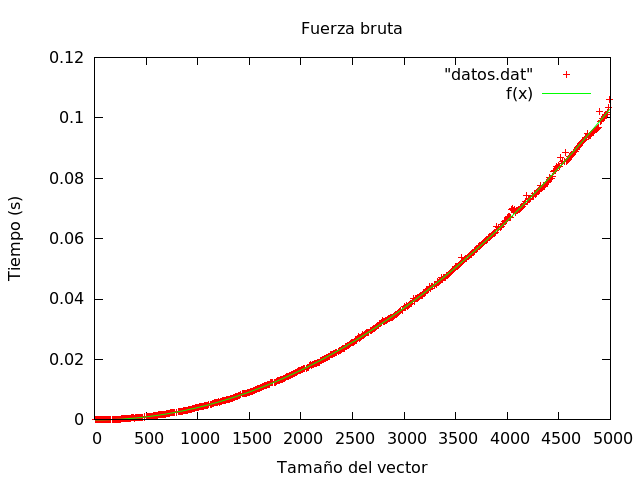
\includegraphics[width=0.6\textwidth]{../Opcional/Graficas/fuerza_bruta_bruno.png}
	\caption{Subproblemas} 
	\label{fig:perros} 
\end{figure}

\subsection{Comparaci\'on}
\begin{figure}[htb] 
\centering
	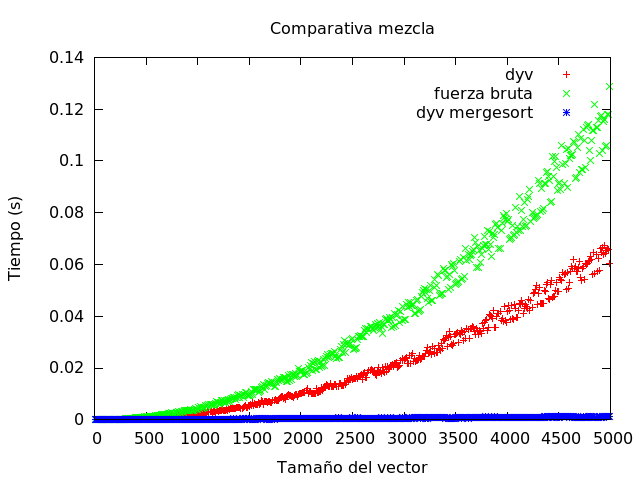
\includegraphics[width=0.6\textwidth]{../Opcional/Graficas/comparativa.png}
	\caption{Subproblemas} 
	\label{fig:perros} 
\end{figure}

